\documentclass{beamer}
\usepackage[utf8]{inputenc}

% packages
\usepackage{physics}
\usepackage{amsfonts, amsmath, amssymb, amsthm}
\usepackage{systeme}
\usepackage[none]{hyphenat}
\usepackage{fancyhdr}
\usepackage{graphicx}
\graphicspath{{./images/}}
\usepackage{float}
\usepackage{siunitx}
\usepackage{esint}
\usepackage{cancel}
\usepackage{mathtools}

% colors
\usepackage{xcolor}
\definecolor{p}{HTML}{FFDDDD}
\definecolor{g}{HTML}{D9FFDF}
\definecolor{y}{HTML}{FFFFCF}
\definecolor{b}{HTML}{D9FFFF}
\definecolor{o}{HTML}{FADECB}
%\definecolor{}{HTML}{}

% \highlight[<color>]{<stuff>}
\newcommand{\highlight}[2][p]{\mathchoice%
  {\colorbox{#1}{$\displaystyle#2$}}%
  {\colorbox{#1}{$\textstyle#2$}}%
  {\colorbox{#1}{$\scriptstyle#2$}}%
  {\colorbox{#1}{$\scriptscriptstyle#2$}}}%

% paragraph indentation/spacing
\setlength{\parindent}{0cm}
\setlength{\parskip}{5pt}
\renewcommand{\baselinestretch}{1.25}

\newcommand{\br}[1]{\left(#1\right)}
\newcommand{\sbr}[1]{\left[#1\right]}
\newcommand{\cbr}[1]{\left\{#1\right\}}

\DeclareMathOperator{\lcm}{lcm}
\DeclareMathOperator{\im}{im}

\usetheme{Madrid}
\usecolortheme{default}

%------------------------------------------------------------
%This block of code defines the information to appear in the title page
\title[The Smith normal form] %optional
{The Smith normal form}

\subtitle{and its use in computing simplicial homology}

\author[Sai Sivakumar] % (optional)
{Sai Sivakumar}

\AtBeginSection[]{
  \begin{frame}
  \vfill
  \centering
  \begin{beamercolorbox}[sep=8pt,center,shadow=true,rounded=true]{title}
    \usebeamerfont{title}\insertsectionhead\par%
  \end{beamercolorbox}
  \vfill
  \end{frame}
}

\begin{document}

%The next statement creates the title page.
\frame{\titlepage}

%This block of code is for the table of contents after the title page
\begin{frame}
\frametitle{outline}
\tableofcontents
\end{frame}

\section{the Smith normal form}

\begin{frame}
  \frametitle{what the Smith normal form is}

  \begin{theorem}[Smith normal form]
    Let $R$ be a principal ideal domain and let $A$ be an $m\times n$ matrix with entries from $R$.
    
    There exist invertible $m\times m$ and $n\times n$ matrices $U$ and $V$ respectively such that $UAV = S$, where \[S = \left(\begin{array}{ccc|ccc}
      a_1 &  &  &  &  &\\
       & \ddots &  &  &0 &\\
       &  & a_k &  & \\
       \hline
       & 0 &  &  &0
    \end{array}\right)\] and $a_1\mid a_2\mid \cdots \mid a_k$. The $a_i$ are unique up to associates.
  \end{theorem}

\end{frame}

\subsection{proof of existence for Euclidean domains}

\begin{frame}
  \frametitle{proof of existence for Euclidean domains}

  Let $R$ be a Euclidean domain and let $A$ be an $m\times n$ matrix with entries from $R$.

  The following elementary row/column operations on $A$ may be achieved by multiplication on the left/right by invertible (``elementary'') matrices: \begin{enumerate}
    \item Exchanging rows $j$ and $k$
    \item Multiplying row $i$ by any unit of $R$.
    \item Add $q\cdot \text{row } j$ to row $k$ for $q\in R$ and $j\neq k$
  \end{enumerate}
  Same operations for columns in place of rows.
\end{frame}

\begin{frame}
  \frametitle{}

  Let $A$ be a nonzero matrix (every zero matrix is in Smith normal form) with \[A = \begin{pmatrix}
    a_{11} &\cdots &a_{1n}\\
    \vdots &\ddots &\vdots\\
    a_{m1} &\cdots & a_{mn}
  \end{pmatrix}.\] We want to transform this matrix by way of elementary row/column operations into a matrix $A^{\prime}$ with $A^{\prime}_{11}\mid A^{\prime}_{ij}$ for $1\leq i\leq m$ and $1\leq j \leq n$.
  
  
  That is, the first entry of $A^{\prime}$ divides every other entry of $A^{\prime}$.

\end{frame}

\begin{frame}
  \frametitle{}

  Let $\alpha(A)\coloneqq\min\cbr{N(a_{ij})\colon a_{ij}\neq 0_R}$, and call any entry $a_{ij}$ a \textit{minimal entry} if $N(a_{ij}) = \alpha(A)$. We show that $\alpha(A)$ may be decreased by elementary row/column operations if and only if a minimal entry does not divide every entry in $A$:

  If a minimal entry $a_{ij}$ does not divide every entry in $A$, we first handle the case where $a_{ij}$ does not divide an entry $a_{ik}$ for $j\neq k$ (another entry in its row). 

\end{frame}

\begin{frame}
  \frametitle{}

  By the division algorithm on $R$ we have $a_{ik} = qa_{ij} + r$ for $q,r\in R$ with $0<N(r)<N(a_{ij})$.

  Then we can add $-q\cdot\text{column } j$ to column $k$ to form a new matrix $A^{\prime}$ with $\alpha(A^{\prime})$ being at most $N(r)$ since one of its entries is $r = a_{ik} - qa_{ij}$. But $\alpha(A^{\prime}) = N(r)<N(a_{ij})$, which means we have decreased $\alpha(A)$.

  A similar procedure can be done if $a_{ij}$ does not divide another entry in its column.

\end{frame}

\begin{frame}
  \frametitle{}

  If $a_{ij}$ divides entries in its row and column but does not divide an entry found outside of its row and column, say $a_{sk}$ for $i\neq s,j\neq k$, we can reduce the situation to one from before.

  Use elementary row/column operations to achieve the following picture:
  \[\begin{matrix}
    a_{ij} & \cdots & a_{ik}\\
    \vdots & & \vdots \\
    a_{sj} & \cdots & a_{sk}
  \end{matrix}\to \begin{matrix}
    a_{ij} & \cdots & a_{ik}\\
    \vdots & & \vdots \\
    0 & \cdots & a_{sk} -q a_{ik}
  \end{matrix}\to\begin{matrix}
    a_{ij} & \cdots & a_{sk} +(1-q) a_{ik}\\
    \vdots & & \vdots \\
    0 & \cdots & a_{sk} -q a_{ik}
  \end{matrix}\]
  Now $a_{ij}$ does not divide an element in its row, which we already handled.

\end{frame}

\begin{frame}
  \frametitle{}

  We show the converse by the contrapositive.
  
  If a minimal entry $a_{ij}$ does divide every entry in $A$, then $a_{ij}$ divides all entries in any matrix $A^{\prime}$ obtained by applying elementary row/column operations to $A$. As a result, there is no way to reduce $N(a_{ij}) = \alpha(A)$.

\end{frame}

\begin{frame}
  \frametitle{}

  Hence we can take a matrix \[A = \begin{pmatrix}
    a_{11} &\cdots &a_{1n}\\
    \vdots &\ddots &\vdots\\
    a_{m1} &\cdots & a_{mn}
  \end{pmatrix}\] and by elementary row/column operations form a matrix \[A^{\prime} = \begin{pmatrix}
    a_{11}^{\prime} &\cdots &a_{1n}^{\prime}\\
    \vdots &\ddots &\vdots\\
    a_{m1}^{\prime} &\cdots & a_{mn}^{\prime}
  \end{pmatrix}\] with $a_{11}^{\prime}$ dividing all entries of $A^{\prime}$.

\end{frame}

\begin{frame}
  \frametitle{}

  By using more elementary row/column operations form another matrix \[B = \left(\begin{array}{c|ccc}
    a_{11}^{\prime} & 0 &\cdots &0\\
    \hline
    0 & a_{22}^{\prime} & \cdots & a_{2n}^{\prime}\\
    \vdots & \vdots &\ddots &\vdots\\
    0 & a_{m2}^{\prime} & \cdots & a_{mn}^{\prime}
  \end{array}\right) = \left(\begin{array}{c|ccc}
    a_{11}^{\prime} & 0\\
    \hline
    0 & B^{\prime} 
  \end{array}\right).\]

  By induction the smaller matrix $B^{\prime}$ can be made into Smith normal form.

  Hence there exist invertible matrices $U,V$ such that \[UAV = S =\left(\begin{array}{ccc|ccc}
    a_1 &  &  &  &  &\\
     & \ddots &  &  &0 &\\
     &  & a_k &  & \\
     \hline
     & 0 &  &  &0
  \end{array}\right). \]

\end{frame}

\begin{frame}
  \frametitle{}

  The divisibility relations $a_1\mid a_2\mid \cdots \mid a_k$ come from the fact that in $B$, $a_{11}^{\prime}$ divided every entry of $B^{\prime}$. As a result, $a_{11}^{\prime}$ will divide every entry of a matrix obtained by applying row/column operations to $B^{\prime}$. 

  Uniqueness of the Smith normal form up to associates comes from the fact that divisibility holds up to associates.

\end{frame}

\subsection{proof of existence for PIDs}

\begin{frame}
  \frametitle{proof of existence for PIDs}

  We need a few lemmas. Let $R$ be a principal ideal domain, and let $x,y$ be nonzero elements of $R$. \begin{enumerate}
    \item There exists an invertible matrix $W$ such that \[W\begin{pmatrix}
      x \\ y
    \end{pmatrix} = \begin{pmatrix}
      \gcd(x,y) \\ 0
    \end{pmatrix}.\]
    \item There exist invertible matrices $U,V$ such that \[U\begin{pmatrix}
      x & 0 \\ 0 & y
    \end{pmatrix}V = \begin{pmatrix}
      \gcd(x,y) & 0 \\ 0 & \lcm(x,y)
    \end{pmatrix},\] with $\lcm(x,y) \coloneqq xy/\gcd(x,y)$.
  \end{enumerate}
  
\end{frame}

\begin{frame}
  \frametitle{}

  \begin{enumerate}
    \item Since $R$ is a PID, $(x,y) = (d)$ with $d$ associate to $\gcd(x,y)$. Without loss of generality, take $d = \gcd(x,y)$. Thus there exist $\alpha, \beta\in R$ with $\alpha x + \beta y = d$. Since $d\mid x$ and $d\mid y$ there exist $p,q\in R$ with $x = dp$ and $y = dq$. It also follows that $\alpha p + \beta q  = 1_R$.
    
    Take \[W = \begin{pmatrix}
      \alpha & \beta \\ -q & p
    \end{pmatrix}.\] It follows that \[W\begin{pmatrix}
      x \\ y
    \end{pmatrix} = \begin{pmatrix}
      \gcd(x,y) \\ 0
    \end{pmatrix}\] with $\det(W) = 1_R$.
  \end{enumerate}

\end{frame}

\begin{frame}
  \frametitle{}

  \begin{enumerate}
    \setcounter{enumi}{1}
    \item Let $d,\alpha,\beta,p,q$ be given as before. Then with 
    %\begin{pmatrix}
    %  1 & 0 \\ -bq & 1
    %\end{pmatrix}\begin{pmatrix}
    %  1 & 1 \\ 0 & 1
    %\end{pmatrix} =
    \[U = \begin{pmatrix}
      1 & 1 \\ -bq & 1-bq
    \end{pmatrix}, \quad V = \begin{pmatrix}
      a & -q \\ b & p
    \end{pmatrix},\] it follows that \[U\begin{pmatrix}
      x & 0 \\ 0 & y
    \end{pmatrix} V = \begin{pmatrix}
      \gcd(x,y) & 0 \\ 0 & \lcm(x,y)
    \end{pmatrix}\] with $\det(U) = \det(V) = 1_R$. 

  \end{enumerate}

\end{frame}

\begin{frame}
  \frametitle{}

  Another lemma: Let $R$ be a (commutative) Noetherian ring and let $D$ be a nonempty subset of $R$. Show that there exists an element $d\in D$ which is ``minimal with respect to division''; that is, if there exists $d^{\prime}\in D$ with $d^{\prime}\mid d$ then $d\mid d^{\prime}$ also.

\end{frame}

\begin{frame}
  \frametitle{}

  To prove this lemma we must recall what a Noetherian ring is.
  
  A Noetherian ring is one which satisfies the ascending chain condition: For any increasing sequence of ideals $I_1\subseteq I_2\subseteq I_3 \subseteq\cdots$ of $R$ there exists an $n$ such that $I_n = I_{n+1} = \cdots$; that is, the chain stabilizes.

  This is equivalent to the ``maximal principle'': Every nonempty subset of ideals of $R$ has a maximal element.

  Observe that the maximal principle implies the ascending chain condition pretty quickly, but the converse requires Zorn's lemma.

\end{frame}

\begin{frame}
  \frametitle{}

  By taking the set of ideals $\cbr{(a)\colon a\in D}$ and invoking the fact that $R$ is Noetherian we obtain a maximal ideal $(d)$ for some $d\in D$ which satisfies the property we want:
  
  If there is some $d^{\prime}\in D$ with $d^{\prime}\mid d$, we have that $(d)\subseteq (d^{\prime})$. But by maximality of $(d)$ we must have $(d)= (d^{\prime})$ which yields that $d\mid d^{\prime}$ as desired.

\end{frame}

\begin{frame}
  \frametitle{the proof}

  With the lemmas proven we may continue with the proof.

  Let $R$ be a PID (so $R$ is Noetherian), and let $A$ be a matrix with entries from $R$. 

  Let $D$ be given by the set of all entries appearing in \textit{any} matrix $B$ \textit{similar} to $A$, and let $d$ be an element of $D$ which is minimal with respect to division in the sense of the previous lemma.

\end{frame}

\begin{frame}
  \frametitle{}

  Let $A^{\prime}$ be a matrix similar to $A$ such that $d$ appears as the first entry; here $A^{\prime} = U^{\prime}AV^{\prime}$ for invertible $U^{\prime},V^{\prime}$.
  
  We show that $d$ divides every entry in the matrix $A^{\prime}$.

  Suppose some entry $a_{sk}$ does not divide $d$. We can modify one of the first two lemmas to obtain matrices $S,T$ such that $SA^{\prime}T$ contains $\gcd(d,a_{sk})$ as an entry. But $\gcd(d,a_{sk})\mid d$, and since $d$ was chosen minimally with respect to division, it follows that $d\mid \gcd(d,a_{sk})$, from which it follows that $d$ divides $a_{sk}$. Contradiction.

\end{frame}

\begin{frame}
  \frametitle{}

  Since $d$ divides every entry in $A^{\prime}$, we may apply elementary row/column operations to reduce $A^{\prime}$ into a matrix \[B = \left(\begin{array}{c|c}
    d & 0\\\hline 0 & B^{\prime}
  \end{array}\right)\] where $d$ divides every entry in $B^{\prime}$. By induction reduce $B^{\prime}$ to Smith normal form to obtain the result.

  The divisibility relations hold since $d$ divided every entry of $B^{\prime}$ and will divide every entry of a matrix obtained by applying elementary row/column operations to $B^{\prime}$.

  The Smith normal form is unique up to associates since divisibility holds up to associates.

\end{frame}

\section{some computational remarks}

\begin{frame}
  \frametitle{the row reduction algorithm}

  For integer matrices the basic algorithm is just Gaussian elimination (or just the elementary row/column operations we saw earlier).

  Sample pseudocode for reducing $\mathbb{Z}/2\mathbb{Z}$-valued $n_{p-1}\times n_p$ matrices: \begin{figure}[h]
    \centering
    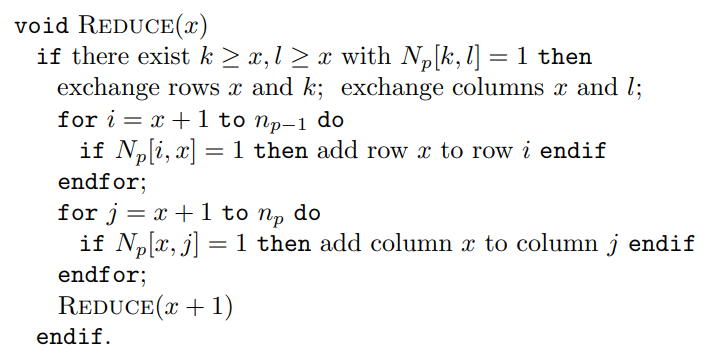
\includegraphics[scale=0.70]{z2algo.PNG}
  \end{figure}

\end{frame}

\begin{frame}
  \frametitle{}

  In each recursive call there are at most $(n_{p-1} + n_p)$ elementary row/column operations so the number of elementary operations is at most $(n_{p-1} + n_p)\min\cbr{n_{p-1} , n_p}$.
  
  By accounting for the length of the columns/rows in the matrix the computational complexity is bounded above by a cubic polynomial in $n_{p-1},n_p$.

\end{frame}

\begin{frame}
  \frametitle{recent-ish results}

  Dumas, Heckenbach, Saunders, and Welker various efficient Smith normal form algorithms \hyperlink{https://membres-ljk.imag.fr/Jean-Guillaume.Dumas/Publications/DHSW.pdf}{\color{blue}{\texttt{link}}}

  Storjohann and Labahn fast Las Vegas algorithm for polynomial matrices \hyperlink{https://cs.uwaterloo.ca/~glabahn/Papers/arne3.pdf}{\color{blue}{\texttt{link}}}

\end{frame}

\section{application to computing simplicial homology}

\begin{frame}
  \frametitle{chain complexes}

  Recall that a \textit{chain complex} $\mathcal{C}$ is a sequence \[\cdots\overset{\partial_{n+2}}{\longrightarrow} C_{n+1} \overset{\partial_{n+1}}{\longrightarrow}C_n\overset{\partial_{n}}{\longrightarrow} C_{n-1}\overset{\partial_{n-1}}{\longrightarrow}\cdots \] of abelian groups $C_i$ with homomorphisms $\partial_i$ such that $\partial_i\circ\partial_{i+1} = 0$.

  We define the \textit{homology groups} by $H_i(\mathcal{C}) = \ker\partial_i/\im\partial_{i+1}$.

\end{frame}

\begin{frame}
  \frametitle{standard bases for free chain complexes}

  When the groups $C_i$ of a chain complex are free of finite rank, there exist subgroups $U_i,V_i,W_i$ of $C_i$ such that \[C_i = U_i\oplus V_i\oplus W_i\] where $\partial_i(U_i)\subseteq W_{i-1}$ and $\partial_i(V_i) = \partial_i(W_i) = 0$

\end{frame}

\begin{frame}
  \frametitle{}

  \textit{Step 1}: let $W_i$ be the set of all elements $c$ of $C_i$ such that some nonzero multiple of $c$ is found in $\im \partial_{i+1}$. Check that $W_i$ is a subgroup of $C_i$.

  The following containments hold:
  \[\im \partial_{i+1}\subseteq W_i\subseteq \ker\partial_i \subseteq C_i\] The second containment holds since $C_i$ is torsion free, from which $mc_i = \partial_{i+1}d_{i+1}$ yields $\partial_i c_i = 0$.

\end{frame}

\begin{frame}
  \frametitle{}

  To show that $W_i$ is a direct summand of $\ker \partial_i$, consider the natural projection \[\ker\partial_i \to H_i(\mathcal{C})\to H_i(\mathcal{C})/T_i(\mathcal{C})\] where $T_i(\mathcal{C})$ is the torsion subgroup of $H_i(\mathcal{C})$.

  An element $c\in \ker\partial_i$ is in the kernel of this projection if and only if some multiple of $c$ is in $\im\partial_{i+1}$; i.e., if $c\in W_i$. Hence \[\ker\partial_i/W_i \cong H_i(\mathcal{C})/T_i(\mathcal{C}),\] and since $H_i(\mathcal{C})/T_i(\mathcal{C})$ is finitely generated and torsion-free, it is free.

\end{frame}

\begin{frame}
  \frametitle{}

  It follows that $\ker\partial_i /W_i$ is free.
  
  If $\cbr{c_1 + W_i,\dots,c_k + W_i}$ is a basis for $\ker\partial_i /W_i$ and $\cbr{d_1,\dots,d_l}$ is a basis for $W_i$, then $\cbr{c_1,\dots,c_k,d_1,\dots,d_l}$ is a basis for $\ker\partial_i$.
  
  It follows that $W_i$ is a direct summand of $\ker\partial_i$, so $\ker\partial_i = V_i \oplus W_i$, where $V_i$ has basis $\cbr{c_1,\dots,c_k}$.

\end{frame}

\begin{frame}
  \frametitle{}

  \textit{Step 2}: Choose ordered bases $\cbr{e_1,\dots,e_n}$ for $C_i$ and $\cbr{d_1,\dots,d_m}$ for $C_{i-1}$ for which the matrix of $\partial_i\colon C_i\to C_{i-1}$ takes on the Smith normal form \[\left(\begin{array}[]{ccc|c}
    b_1 &  &  &   \\
    & \ddots & &0  \\
    & & b_l &  \\
    \hline 
    & 0& & 0 
  \end{array}\right)\] with $b_i\geq 1$ and $b_1\mid b_2\mid\cdots\mid b_l$.

\end{frame}

\begin{frame}
  \frametitle{}

  The following hold: \begin{enumerate}
    \item $\cbr{e_{l+1},\dots,e_n}$ is a basis for $\ker\partial_i$.
  \end{enumerate}

  Observe $<e_{l+1},\dots,e_n>\subseteq \ker\partial_i$ and if we take any element $c = \sum_{k=1}^n a_ke_k\in C_i$ then $\partial_i( c) = \sum_{k=1}^lb_ka_kd_k$. 
  
  For $c$ to be in $\ker\partial_i$ we must have $\partial_i(c) = 0$; equivalently, $a_1,\dots,a_l$ must be zero, and in this case $c = \sum_{k=l+1}^n a_ke_k$.

\end{frame}

\begin{frame}
  \frametitle{}
  
  \begin{enumerate}
    \setcounter{enumi}{1}
    \item $\cbr{d_1,\dots,d_l}$ is a basis for $W_{i-1}$. 
  \end{enumerate}
  To show the second point, observe that $d_1,\dots,d_l\in W_{i-1}$ since $b_kd_k = \partial_i(e_k)$ for $1\leq k \leq l$. 

  Conversely, let $f = \sum_{k=1}^m f_kd_k\in C_{i-1}$, and if $f\in W_{i-1}$, then for some $\lambda\neq 0$ and $c =\sum_{k=1}^n a_ke_k\in C_i$ we have \[\lambda f = \sum_{k=1}^m \lambda f_kd_k = \partial_i(c) = \sum_{k=1}^lb_ka_kd_k.\] It follows that $f_{l+1},\dots,f_m = 0$ so that $f\in <d_1,\dots,d_l>$ as well.

\end{frame}

\begin{frame}
  \frametitle{}

  \begin{enumerate}
    \setcounter{enumi}{2}
    \item $\cbr{b_1d_1,\dots,b_ld_l}$ is a basis for $\im\partial_i$.
  \end{enumerate}
  The third point holds since any element of $\im\partial_i$ is in the form $\sum_{k=1}^lb_ka_kd_k$ which is in $<b_1d_1,\dots,b_ld_l>$. The reverse containment also holds, and $\cbr{b_1d_1,\dots,b_ld_l}$ is linearly independent since $b_k\geq 1 $.

\end{frame}

\begin{frame}
  \frametitle{}

  \textit{Step 3}: To prove the theorem, choose ordered bases for $C_i$ and $C_{i-1}$ as in Step 2 and choose $U_i$ to be the group generated by $\cbr{e_1,\dots,e_l}$ so that \[C_i = U_i\oplus \ker\partial_i.\] By Step 1, decompose $\ker\partial_i$ into $V_i\oplus W_i$ so that \[C_i = U_i\oplus V_i\oplus W_i.\] We obtain also that $\partial_i(U_i)\subseteq W_{i-1}$ and $\partial_i(V_i) = \partial_i(W_i) = 0$. Carrying out Step 2 in full gives us the required bases for $U_i$ and $W_{i-1}$.

\end{frame}

\begin{frame}
  \frametitle{computing homology groups}

  The homology groups of a finite simplicial complex $K$ can be computed explicitly.

  Orient the simplices of $K$ and obtain the groups $C_i$ and maps $\partial_i$ forming a chain complex $\mathcal{C}$. Use the previous result to decompose $C_p$ as $U_p\oplus V_p \oplus W_p$.

\end{frame}

\begin{frame}
  \frametitle{}

  Then\begin{multline*}
    H_p(\mathcal{C}) = \ker\partial_p/\im\partial_{p+1} \cong (V_p\oplus W_p)/\im\partial_{p+1} \\= V_p\oplus (W_p/\im\partial_{p+1})\cong (\ker\partial_p/W_p)\oplus(W_p/\im\partial_{p+1}).
  \end{multline*} The first group in the direct sum is free and the second group is a torsion group.

  We have thus reduced computing homology to computing these two groups.

\end{frame}

\begin{frame}
  \frametitle{}

  Take the matrices of $\partial_p\colon C_p\to C_{p-1}$ and $\partial_{p+1}\colon C_{p+1}\to C_p$ (which will have entries from $\cbr{0,1,-1}$) and reduce them to Smith normal forms $S_p,S_{p+1}$, respectively.
  
  Let $b_1,\dots,b_l$ be the nonzero entries appearing in the diagonal of $S_{p+1}$.

  Then \begin{enumerate}
    \item The rank of $\ker\partial_p$ is equal to the number of zero \textit{columns} of $S_p$.
    \item The rank of $W_{p-1}$ is equal to the number of nonzero \textit{rows} of $S_p$.
    \item There is an isomorphism \[W_p/\im\partial_{p+1}\cong \mathbb{Z}/b_1\mathbb{Z}\oplus\mathbb{Z}/b_2\mathbb{Z}\oplus\cdots\oplus\mathbb{Z}/b_l\mathbb{Z}\]
  \end{enumerate}

\end{frame}

\begin{frame}
  \frametitle{sources}

  Munkres algebraic topology

  Dummit and Foote algebra

  Professor Speyer's (UMich LSA) worksheets from most recent Algebra class \hyperlink{https://dept.math.lsa.umich.edu/~speyer/593/593_Worksheets_2021_Public.pdf}{\color{blue}{\texttt{link}}}

  Edelbrunner and Harer computational topology

\end{frame}

\end{document}